\documentclass[aspectratio=169]{beamer}
\usepackage[utf8]{inputenc}
\usepackage[T1]{fontenc}
\usepackage[brazil]{babel}
\usepackage{ragged2e}
\usepackage{booktabs}
\usepackage{verbatim}
\usepackage{gensymb}
\usepackage{multirow}
\usepackage{xcolor,colortbl}
\definecolor{verde}{rgb}{0,0.5,0}
\usepackage{listings}
\lstset{
  language=C++,
  basicstyle=\ttfamily\small,
  keywordstyle=\color{blue},
  stringstyle=\color{verde},
  commentstyle=\color{red},
  extendedchars=true,
  showspaces=false,
  showstringspaces=false,
%  numbers=left,
%  numberstyle=\tiny,
  breaklines=true,
  backgroundcolor=\color{green!10},
  breakautoindent=true,
  captionpos=b,
  xleftmargin=0pt
}
\newcommand\setItemnumber[1]{\setcounter{enumi}{\numexpr#1-1\relax}}

\usetheme{AnnArbor}
\usecolortheme{orchid}
\usefonttheme[onlymath]{serif}

\AtBeginSection[]{
  \begin{frame}
  \vfill
  \centering
  \begin{beamercolorbox}[sep=8pt,center,shadow=true,rounded=true]{title}
    \usebeamerfont{title}\insertsectionhead\par%
  \end{beamercolorbox}
  \vfill
  \end{frame}
}

\title[\sc{Classes e Objetos}]{Classes e Objetos}
\author[Roland Teodorowitsch]{Roland Teodorowitsch}
%\institute[LP2 - EC - PUCRS]{Laboratório de Programação II - Curso de Engenharia de Computação - PUCRS}
\institute[POO - EC - PUCRS]{Programação Orientada a Objetos - ECo - Curso de Engenharia de Computação - PUCRS}
\date{8 de junho de 2022}

\begin{document}
\justifying

%-------------------------------------------------------
\begin{frame}
	\titlepage
\end{frame}

%=======================================================
\section{Motivação}

%-------------------------------------------------------
\begin{frame}\frametitle{Um Sistema para Gestão Escolar}

\begin{table}[]
\scriptsize{
\begin{tabular}{|l|l|l|l|l|l|}
\hline
\multicolumn{1}{|c|}{\multirow{2}{*}{\textbf{Dados (Atributos)}}} & \multicolumn{5}{c|}{\textbf{Funções (Métodos)}} \\ \cline{2-6} 
\multicolumn{1}{|c|}{} & mediaIdade() & mediaAprovados() & imprimeAlunos() & calculaSalario() & imprimeProfs() \\
\hline
String nomeAlunos{[}10{]} &  &  &  &  &  \\
\hline
int idadeAlunos{[}10{]} &  &  &  &  &  \\
\hline
float notas{[}10{]}{[}3{]} &  &  &  &  &  \\
\hline
float HORA\_AULA=35 &  &  &  &  &  \\
\hline
string nomeProfs{[}5{]} &  &  &  &  &  \\
\hline
float salarioProfs{[}5{]} &  &  &  &  &  \\
\hline
int nTurmas{[}5{]} &  &  &  &  &  \\
\hline
\end{tabular}
}
\end{table}
\end{frame}

%-------------------------------------------------------
\begin{frame}\frametitle{Um Sistema para Gestão Escolar}

\begin{table}[]
\scriptsize{
\begin{tabular}{|l|l|l|l|l|l|}
\hline
\multicolumn{1}{|c|}{\multirow{2}{*}{\textbf{Dados (Atributos)}}} & \multicolumn{5}{c|}{\textbf{Funções (Métodos)}} \\ \cline{2-6} 
\multicolumn{1}{|c|}{} & mediaIdade() & mediaAprovados() & imprimeAlunos() & calculaSalario() & imprimeProfs() \\
\hline
String nomeAlunos{[}10{]} &  &  & \multicolumn{1}{c|}{\textbf{X}} &  &  \\
\hline
int idadeAlunos{[}10{]} & \multicolumn{1}{c|}{\textbf{X}} &  & \multicolumn{1}{c|}{\textbf{X}} &  &  \\
\hline
float notas{[}10{]}{[}3{]} &  & \multicolumn{1}{c|}{\textbf{X}} & \multicolumn{1}{c|}{\textbf{X}} &  &  \\
\hline
float HORA\_AULA=35 &  &  &  & \multicolumn{1}{c|}{\textbf{X}} &  \\
\hline
string nomeProfs{[}5{]} &  &  &  &  & \multicolumn{1}{c|}{\textbf{X}} \\
\hline
float salarioProfs{[}5{]} &  &  &  & \multicolumn{1}{c|}{\textbf{X}} & \multicolumn{1}{c|}{\textbf{X}} \\
\hline
int nTurmas{[}5{]} &  &  &  & \multicolumn{1}{c|}{\textbf{X}} &  \\
\hline
\end{tabular}
}
\end{table}
\end{frame}

%-------------------------------------------------------
\begin{frame}\frametitle{Um Sistema para Gestão Escolar}

\begin{table}[]
\scriptsize{
\begin{tabular}{|l|l|l|l|l|l|}
\hline
\multicolumn{1}{|c|}{\multirow{2}{*}{\textbf{Dados (Atributos)}}} & \multicolumn{5}{c|}{\textbf{Funções (Métodos)}} \\ \cline{2-6} 
\multicolumn{1}{|c|}{} & mediaIdade() & mediaAprovados() & imprimeAlunos() & calculaSalario() & imprimeProfs() \\
\hline
String nomeAlunos{[}10{]} &  &  & \multicolumn{1}{c|}{\cellcolor{blue!25}\textbf{X}} &  &  \\
\hline
int idadeAlunos{[}10{]} & \multicolumn{1}{c|}{\cellcolor{blue!25}\textbf{X}} &  & \multicolumn{1}{c|}{\cellcolor{blue!25}\textbf{X}} &  &  \\
\hline
float notas{[}10{]}{[}3{]} &  & \multicolumn{1}{c|}{\cellcolor{blue!25}\textbf{X}} & \multicolumn{1}{c|}{\cellcolor{blue!25}\textbf{X}} &  &  \\
\hline
float HORA\_AULA=35 &  &  &  & \multicolumn{1}{c|}{\cellcolor{green!25}\textbf{X}} &  \\
\hline
string nomeProfs{[}5{]} &  &  &  &  & \multicolumn{1}{c|}{\cellcolor{green!25}\textbf{X}} \\
\hline
float salarioProfs{[}5{]} &  &  &  & \multicolumn{1}{c|}{\cellcolor{green!25}\textbf{X}} & \multicolumn{1}{c|}{\cellcolor{green!25}\textbf{X}} \\
\hline
int nTurmas{[}5{]} &  &  &  & \multicolumn{1}{c|}{\cellcolor{green!25}\textbf{X}} &  \\
\hline
\end{tabular}
}
\end{table}
\end{frame}

%=======================================================
\section{Objetos e Classes}

%-------------------------------------------------------
\begin{frame}\frametitle{Objeto}
\begin{itemize}
	\item Um objeto refere-se a uma coisa do mundo
	\item Agrupa dados e funções correlatas
	\item Constituído por atributos e métodos
	\item Atributos são os dados (variáveis de instância)
	\item Métodos são funções e procedimentos
	\begin{itemize}
		\item Operam sobre atributos
		\item Definem o comportamento do objeto
	\end{itemize}
\end{itemize}
\end{frame}

%-------------------------------------------------------
\begin{frame}[fragile]\frametitle{Exemplos de Objetos}
\begin{itemize}
	\item Em C++, \texttt{string} é uma classe
\begin{lstlisting}
string str = "Strings em C++ sao objetos";
cout << str.length() << endl;
\end{lstlisting}
	\item Objetos criados a partir de uma classe chamada \texttt{Aluno}
\begin{lstlisting}
Aluno a1;
a1.defineNome("Joao Souza");

Aluno *a2 = new Aluno("Paula da Silva");
cout << a2->obtemNome() << endl;
delete a2;
\end{lstlisting}
\end{itemize}
\end{frame}

%-------------------------------------------------------
\begin{frame}\frametitle{Classe}
\begin{columns}[T]
\begin{column}{0.5\linewidth}
\begin{itemize}
	\item Uma classe descreve um conjunto de objetos com mesmo comportamento
	\item Objetos não são programados individualmente
	\item O programador escreve classes
	\item Objetos são instâncias de suas classes
	\item Uma classe descreve atributos e métodos de um conjunto de objetos
\end{itemize}
\end{column}
\begin{column}{0.5\linewidth}
\begin{figure}[h]
	\centering
	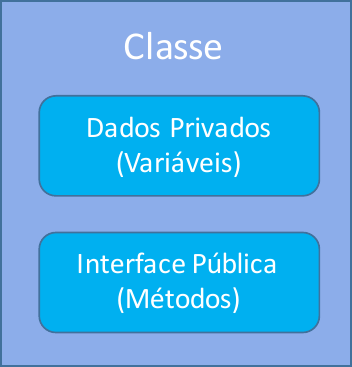
\includegraphics[height=0.45\paperheight]{pucrs-ec-poo-unidade_04-classes_e_objetos-laminas-classe.png}
\end{figure}
\end{column}
\end{columns}
\end{frame}

%-------------------------------------------------------
\begin{frame}\frametitle{Resumo}
\begin{itemize}
	\item \textbf{Objetos} representam coisas do mundo
	\begin{itemize}
		\item Têm atributos e métodos
	\end{itemize}
	\item \textbf{Classes} especificam objetos
	\begin{itemize}
		\item Definem atributos e métodos
	\end{itemize}
\end{itemize}
\end{frame}

%-------------------------------------------------------
\begin{frame}\frametitle{Resumo}
\begin{itemize}
	\item \textbf{Objetos} têm um estado interno e ...
	\begin{itemize}
		\item Valores atuais de seus atributos
	\end{itemize}
	\item ... uma interface pública.
	\begin{itemize}
		\item Conjunto de métodos para manipulação do estado interno
	\end{itemize}
	\item Interface pública encapsula estado interno
	\begin{itemize}
		\item Esconde detalhes de implementação
	\end{itemize}
	\item \textbf{Classe} define como são estruturados o estado interno e a interface pública (e sua implementação)
\end{itemize}
\end{frame}

%=======================================================
\section{Implementando uma Classe Simples}

%-------------------------------------------------------
\begin{frame}\frametitle{Classe Contador}
\begin{columns}[T]
\begin{column}{0.5\linewidth}
\begin{itemize}
	\item Uma classe que modela um dispositivo mecânico que é usado para realizar contagens
	\begin{itemize}
		\item Por exemplo, para contar quantas pessoas estão assistindo a um concerto ou quantas pessoas embarcaram em um ônibus
	\end{itemize}
	\item O que deve ser feito?
	\begin{itemize}
		\item Incrementar o dispositivo
		\item Obter o valor atual
		\item Zerar o contador
	\end{itemize}
\end{itemize}
\end{column}
\begin{column}{0.5\linewidth}
\begin{figure}[h]
	\centering
	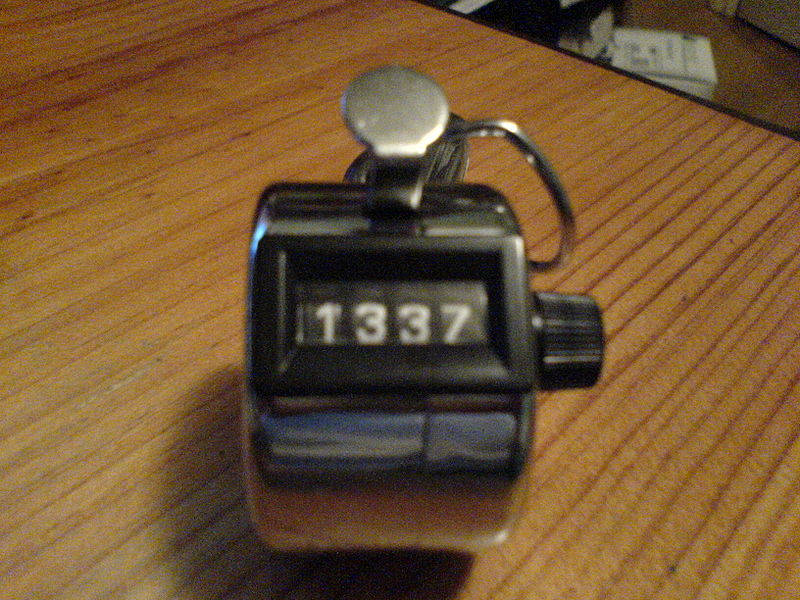
\includegraphics[height=0.45\paperheight]{pucrs-ec-poo-unidade_04-classes_e_objetos-laminas-contador.jpg}
\end{figure}
\end{column}
\end{columns}
\end{frame}

%-------------------------------------------------------
\begin{frame}[fragile]\frametitle{Criando a Classe Contador}
\begin{itemize}
	\item Estrutura
\begin{lstlisting}
class Contador {
  // ...
};
\end{lstlisting}
	\item Atributos
	\item Métodos
	\begin{itemize}
		\item De Acesso (\emph{getters})
		\item De Modificação (\emph{setters})
		\item Construtor(es)
		\item Destrutor
	\end{itemize}
\end{itemize}
\end{frame}

%-------------------------------------------------------
\begin{frame}[fragile]\frametitle{Atributos}
\begin{itemize}
	\item Por enquanto, serão sempre privados
	\item Cada objeto da classe \texttt{Contador} terá a sua cópia dos atributos
\end{itemize}
\begin{lstlisting}
class Contador {
  private:
    int valor;
  // ...
};
\end{lstlisting}
\end{frame}

%-------------------------------------------------------
\begin{frame}[fragile]\frametitle{Métodos de Acesso (\emph{Getters})}
\begin{itemize}
	\item Apenas acessam atributos do objeto, sem alterar o estado interno do objeto
	\item Usualmente retornam UM atributo
	\item Comumente nomeados como ``get'' + AttributeName ou ``obtem'' + NomeAtributo
	\item Raramente apresentam parâmetros e costumam ser públicos
\end{itemize}
\begin{lstlisting}[basicstyle=\ttfamily\scriptsize]
class Contador {
  private:
    int valor;
  public:
    // ...

    int obtemValor() {
      return valor;
    }

    // ...
};
\end{lstlisting}
\end{frame}

%-------------------------------------------------------
\begin{frame}[fragile]\frametitle{Métodos de Modificação (\emph{Setters})}
\begin{itemize}
	\item Modificam atributos do objeto, alterando o estado interno do objeto
	\item Geralmente apresentam um parâmetro e alteram UM atributo do objeto
	\item Normalmente nomeados como ``set'' + AttributeName ou ``define'' + NomeAtributo
	\item Frequentemente o tipo de retorno é \texttt{void} e também costumam ser públicos
\end{itemize}
\begin{lstlisting}[basicstyle=\ttfamily\tiny]
class Contador {
  private:
    int valor;
  public:
    // ...

    void incrementa() {
      valor = valor + 1;
    }

    void defineValor(int v) {
      valor = v;
    }

    // ...
};
\end{lstlisting}
\end{frame}

%-------------------------------------------------------
\begin{frame}\frametitle{Atributos e Métodos}
\begin{itemize}
	\item Observe que:
	\begin{itemize}
		\item \texttt{private:} e \texttt{public:} são modificadores
		\item Por enquanto, vamos usar \texttt{private:} para atributos e \texttt{public:} para métodos
		\item Mas NÃO é raro encontrar métodos \texttt{private:} (são de uso interno)
	\end{itemize}
	\item Objetos sem \emph{setter} são imutáveis
	\item É comum cada atributo ter pelo menos um método \emph{getter} e um método \emph{setter}, mas...
	\item Deve-se evitar criar esses métodos mecanicamente sem verificar se fazem sentido ou NÃO
	\item Deve-se sempre privilegiar métodos de negócio
	\begin{itemize}
		\item Em vez de \texttt{conta.defineSaldo(conta.obtemSaldo() + 100)}
		\item É melhor \texttt{conta.credita(100)}
	\end{itemize}
	\item Dica de leitura: \url{https://blog.caelum.com.br/nao-aprender-oo-getters-e-setters/}
\end{itemize}
\end{frame}

%-------------------------------------------------------
\begin{frame}\frametitle{Método Construtor}
\begin{itemize}
	\item É um método que será chamado quando um objeto da classe for criado (por exemplo, quando se usa o operador \texttt{new})
	\item Constrói objetos, definindo os valores iniciais dos atributos (ou seja, inicializando o estado interno do objeto)
	\item Tem o mesmo nome da classe
	\item NÃO tem tipo de retorno
	\item Geralmente é público
	\item Uma classe pode ter mais de um construtor (sobrecarga)
	\item Se nenhum construtor for declarado, o compilador criará um construtor padrão automaticamente (vazio)
	\begin{itemize}
		\item Ele NÃO receberá nenhum parâmetro
		\item Ele NÃO inicializará as variáveis de instância
	\end{itemize}
\end{itemize}
\end{frame}

%-------------------------------------------------------
\begin{frame}[fragile]\frametitle{Método Construtor}
\begin{columns}[T]
\begin{column}{0.5\linewidth}
\begin{lstlisting}
class Contador {
  private:
    int valor;

  public:
    Contador() {
      valor = 0;
    }

    Contador(int v) {
      valor = v;
    }
\end{lstlisting}
\end{column}
\begin{column}{0.5\linewidth}
\begin{lstlisting}
    int obtemValor() {
      return valor;
    }

    void incrementa() {
      valor = valor + 1;
    }

    void defineValor(int v) {
      valor = v;
    }
};
\end{lstlisting}
\end{column}
\end{columns}
\end{frame}

%-------------------------------------------------------
\begin{frame}[fragile]\frametitle{Construtor com Parâmetros Opcionais}
\begin{itemize}
	\item É possível definir métodos e construtores com valores opcionais (\emph{default})
\end{itemize}
\begin{lstlisting}
class Contador {
  private:
    int valor;

  public:
    Contador(int v = 0) {
      valor = v;
    }

    // ...
};
\end{lstlisting}
\end{frame}

%-------------------------------------------------------
\begin{frame}[fragile]\frametitle{Execução de Construtores}
\begin{itemize}
	\item Objetos podem ser criados como variáveis ou usando o operador \texttt{new}
\end{itemize}
\begin{lstlisting}
int main() {
  Contador c1; // Novo contador com valor inicial 0
  Contador *c2 = new Contador(10); // Contador com valor 10
  c2->incrementa();
  c2->incrementa();
  cout << c2->obtemValor() << endl; // Deve imprimir 12
  delete c2;
  c1.incrementa();
  c1.incrementa();
  c1.incrementa();
  cout << c1.obtemValor() << endl; // Deve imprimir 3
  return 0;
}
\end{lstlisting}
\end{frame}

%-------------------------------------------------------
\begin{frame}[fragile]\frametitle{Construtores -- Erros Comuns}
\begin{itemize}
	\item NÃO inicializar referências a objetos
	\begin{itemize}
		\item \textbf{Referências} são inicializadas por padrão com \texttt{null}
		\item Chamar um método de uma referência que contém \texttt{null} resulta em um erro de execução (\emph{segmentation fault})
	\end{itemize}
\end{itemize}
\begin{lstlisting}
int main() {
  Contador *c2;
  c2->incrementa(); // SEGMENTATION FAULT
  cout << c2->obtemValor() << endl;
  delete c2;
  return 0;
}
\end{lstlisting}
\end{frame}

%-------------------------------------------------------
\begin{frame}[fragile]\frametitle{Construtores -- Erros Comuns}
\begin{itemize}
	\item Tentar chamar um construtor
	\begin{itemize}
		\item NÃO se pode chamar um construtor como é feito com outros métodos
		\item Ele é ``invocado'' automaticamente na declaração de um objeto ou através do operador \texttt{new}
\begin{lstlisting}
Contador c1, c2(10);
Contador *c3 = new Contador();
\end{lstlisting}
		\item NÃO se pode invocar um construtor para um objeto que já existe
\begin{lstlisting}
c1.Contador(); // ERRO
c3->Contador(); // ERRO
\end{lstlisting}
		\item Mas pode-se criar um novo objeto usando uma referência existente
\begin{lstlisting}
Contador *c3 = new Contador();
c3->incrementa();
delete c3;
c3 = new Contador(10);
\end{lstlisting}
	\end{itemize}
\end{itemize}
\end{frame}

%-------------------------------------------------------
\begin{frame}[fragile]\frametitle{Construtores -- Erros Comuns}
\begin{itemize}
	\item Declarar um construtor como \texttt{void}
	\begin{itemize}
		\item Construtores NÃO têm tipo de retorno
	\end{itemize}
\begin{lstlisting}
class Contador {
  private:
    int valor;
  public:
    void Contador() {
      valor = 0;
    }
    // ...
};
\end{lstlisting}
\end{itemize}
\end{frame}

%-------------------------------------------------------
\begin{frame}[fragile]\frametitle{Destrutor}
\begin{itemize}
	\item É um método usado para ``limpeza'' (liberação de recursos) quando um objeto não é mais necessário
	\item NÃO tem parâmetros
	\item Também NÃO tem tipo de retorno
	\item Seu nome corresponde ao nome da classe precedido de um til (\textasciitilde)
	\item É invocado quando um objeto é destruído ou quando uma referência é desalocada (\texttt{delete})
\begin{lstlisting}[basicstyle=\ttfamily\footnotesize]
class Contador {
  // ...
  public:
    ~Contador() {
      cout << "Destrutor de Contador chamado..." << endl;
    }
    // ...
};
\end{lstlisting}
\end{itemize}
\end{frame}

%-------------------------------------------------------
\begin{frame}[fragile]\frametitle{Organizando o Código das Classes}
\begin{itemize}
	\item A declaração de uma classe
	\begin{itemize}
		\item Contém \textbf{atributos privados} e \textbf{métodos públicos}
		\item Deve ser terminada por ponto-e-vírgula (\texttt{;})
	\end{itemize}
\begin{lstlisting}[basicstyle=\ttfamily\footnotesize]
class NomeDaClasse {
  private:
    // atributos
  public:
    // metodos
};        
\end{lstlisting}
	\item É possível incluir a declaração de várias classes em um mesmo arquivo
	\item Também é possível separar \textbf{definição} (que fica em um arquivo \texttt{.hpp}) de \textbf{implementação} (que fica em um arquivo \texttt{.cpp})
\end{itemize}
\end{frame}

%-------------------------------------------------------
\begin{frame}[fragile]\frametitle{Classe com Arquivo de Cabeçalho}
\begin{columns}[T]
\begin{column}{0.35\linewidth}
\begin{lstlisting}[basicstyle=\ttfamily\tiny]
// Contador.hpp
#ifndef _CONTADOR_HPP
#define _CONTADOR_HPP
using namespace std;
class Contador {
  private:
    int valor;
  public:
    Contador(int v = 0);
    ~Contador();
    int obtemValor();
    void incrementa();
    void defineValor(int v);
};
#endif
\end{lstlisting}
\begin{lstlisting}[basicstyle=\ttfamily\tiny]
// main.cpp
#include "Contador.hpp"
#include <iostream>
int main() {
  Contador *c1 = new Contador(10);
  cout << c1->obtemValor() << endl;
  delete c1;
  return 0;
}
\end{lstlisting}
\end{column}
\begin{column}{0.65\linewidth}
\begin{lstlisting}[basicstyle=\ttfamily\scriptsize]
// Contador.cpp
#include <iostream>
#include "Contador.hpp"

Contador::Contador(int v) { // Observar o uso de ::
  valor = v;
}
Contador::~Contador() {
  cout << "Destrutor de Contador chamado..." << endl;
}
int Contador::obtemValor() {
  return valor;
}
void Contador::incrementa() {
  valor = valor + 1;
}
void Contador::defineValor(int v) {
  valor = v;
}
\end{lstlisting}
\end{column}
\end{columns}
\end{frame}

%-------------------------------------------------------
\begin{frame}[fragile]\frametitle{Funções e Métodos Embutidos}
\begin{itemize}
	\item A palavra-chave \texttt{inline} colocada no início da declaração ou da implementação de funções ou métodos, faz com que o compilador substitua a chamada pela própria implementação
	\item Isto torna o programa mais rápido, pois evita a execução da chamada
	\item Um método definido no corpo de uma declaração de classe é implicitamente embutido
\end{itemize}
\begin{lstlisting}[basicstyle=\ttfamily\tiny	]
class Exemplo {
private:
    int valor;
public:
    Exemplo(int v) {
      valor = v;
      cout << "Construtor (implicitamente embutido) chamado..." << endl;
    }
    ~Exemplo();
    int obtemValorNaoEmbutido();
    int obtemValorEmbutido();
};

Exemplo::~Exemplo() {  cout << "Destrutor (NAO embutido) chamado..." << endl;  }

int Exemplo::obtemValorNaoEmbutido() {  return valor;  }

inline int Exemplo::obtemValorEmbutido() {  return valor;  }
\end{lstlisting}
\end{frame}

%=======================================================
\section{Introdução à UML}

%-------------------------------------------------------
\begin{frame}\frametitle{Unified Modeling Language (UML)}
\begin{itemize}
	\item Linguagem para modelagem de sistemas
	\item Visual e abstrata
	\item Diversos tipos de diagramas
	\item Nesta disciplina usaremos Diagrama de classes
\end{itemize}
\end{frame}

%-------------------------------------------------------
\begin{frame}\frametitle{Diagrama de Classes}
\begin{itemize}
	\item  Representação visual de classes
	\item  Classes representadas como caixas
	\item  Atributos e métodos (sem implementação)
\end{itemize}
\begin{figure}[h]
	\centering
	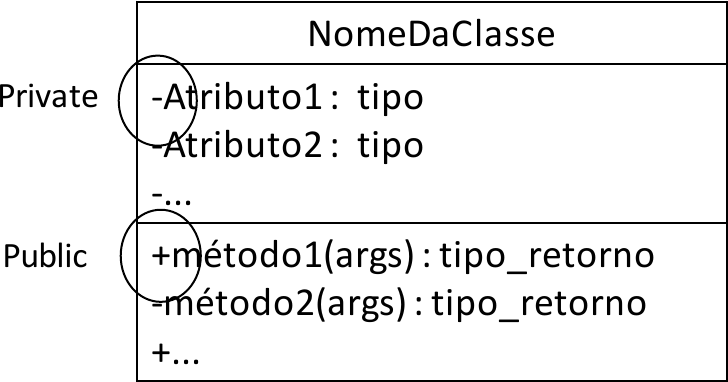
\includegraphics[height=0.45\paperheight]{pucrs-ec-poo-unidade_04-classes_e_objetos-laminas-uml1.png}
\end{figure}
\end{frame}

%-------------------------------------------------------
\begin{frame}[fragile]\frametitle{Exemplo -- Classe Contador}
\begin{columns}[T]
\begin{column}{0.5\linewidth}
\begin{figure}[h]
	\centering
	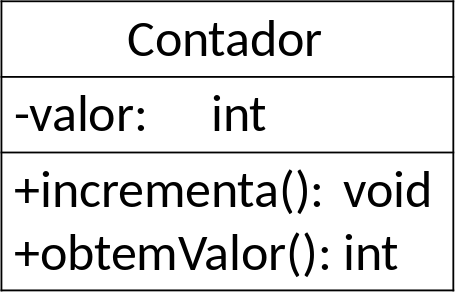
\includegraphics[height=0.3\paperheight]{pucrs-ec-poo-unidade_04-classes_e_objetos-laminas-uml2.png}
\end{figure}
\end{column}
\begin{column}{0.5\linewidth}
\begin{lstlisting}
class Contador {
  private:
    int valor;

  public:
    void incrementa() {
      valor = valor + 1;
    }
    int obtemValor() {
      return valor;
    }
};
\end{lstlisting}
\end{column}
\end{columns}
\end{frame}

%=======================================================
\section{Construindo uma Classe}

%-------------------------------------------------------
\begin{frame}\frametitle{Passos Gerais para Construir uma Classe}
\begin{enumerate}
	\item Definir a interface pública (métodos)
	\item Definir os atributos (dados)
	\item Implementar a interface pública
\end{enumerate}
\end{frame}

%-------------------------------------------------------
\begin{frame}\frametitle{Exemplo -- Caixa Registradora}
\begin{itemize}
	\item Comportamento desejado:
	\begin{itemize}
		\item Adicionar o preço de um item
		\item Pegar o total da venda
		\item Pegar o total de itens vendidos
		\item Limpar o caixa para uma nova venda
	\end{itemize}
\end{itemize}
\begin{figure}[h]
	\centering
	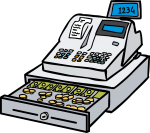
\includegraphics[height=0.4\paperheight]{pucrs-ec-poo-unidade_04-classes_e_objetos-laminas-caixa_registradora.png}
\end{figure}
\end{frame}

%-------------------------------------------------------
\begin{frame}\frametitle{(1) Definindo a Interface Pública (Métodos)}
\begin{figure}[h]
	\centering
	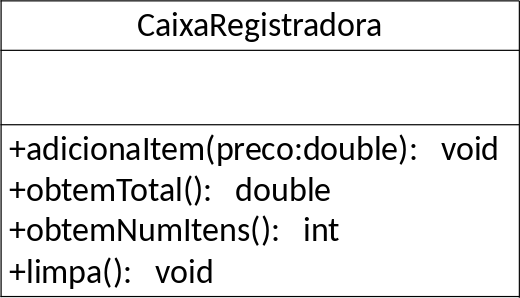
\includegraphics[height=0.5\paperheight]{pucrs-ec-poo-unidade_04-classes_e_objetos-laminas-caixa_registradora1.png}
\end{figure}
\end{frame}

%-------------------------------------------------------
\begin{frame}\frametitle{(2) Definindo Atributos (Dados)}
\begin{figure}[h]
	\centering
	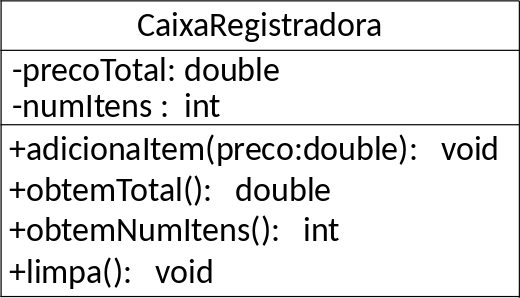
\includegraphics[height=0.5\paperheight]{pucrs-ec-poo-unidade_04-classes_e_objetos-laminas-caixa_registradora2.png}
\end{figure}
\end{frame}

%-------------------------------------------------------
\begin{frame}[fragile]\frametitle{(3) Implementação em 3 arquivos}
\begin{enumerate}
{\scriptsize
	\item \texttt{CaixaRegistradora.hpp}
	\item \texttt{CaixaRegistradora.cpp}
	\item \texttt{main.cpp}
\begin{lstlisting}[basicstyle=\ttfamily\tiny]
#include <iostream>
#include "CaixaRegistradora.hpp"
using namespace std;
int main () {
  CaixaRegistradora * caixa = new CaixaRegistradora ();
  caixa->adicionaItem (1.99); // Adiciona primeiro item
  caixa->adicionaItem (2.99); // Adiciona segundo item
  caixa->adicionaItem (1.50); // Adiciona terceiro item
  cout << caixa->obtemTotal () << endl; // Saida : 6.48
  cout << caixa->obtemNumItens () << endl; // Saida : 3
  caixa->limpa ();
  cout << caixa->obtemTotal () << endl;; // Saida : 0
  cout << caixa->obtemNumItens () << endl; // Saida : 0
  delete caixa;
  CaixaRegistradora caixa2;
  caixa2.adicionaItem(123.456);
  cout << caixa2.obtemTotal() << endl;
  cout << caixa2.obtemNumItens() << endl;
  return 0;
}
\end{lstlisting}
Compilar com: \texttt{g++ -std=c++11 CaixaRegistradora.cpp main.cpp -o executavel}
}
\end{enumerate}
\end{frame}

%=======================================================
\section{Lista de Exercícios 1}

%-------------------------------------------------------
\begin{frame}\frametitle{Lista de Exercícios 1}
\begin{enumerate}
	\item Implementar os arquivos \texttt{CaixaRegistradora.hpp} e \texttt{CaixaRegistradora.cpp} tal como apresentado nos diagramas UML e exemplos das lâminas anteriores.
	\item Crie uma classe para representar uma pessoa, com os seguintes atributos privados: nome, idade e altura. Crie os métodos públicos necessários para acessar estes atributos, alterar estes atributos e também um método para imprimir os dados de uma pessoa.
\end{enumerate}
\end{frame}

%=======================================================
\section{Lista de Exercícios 2}

%-------------------------------------------------------
\begin{frame}\frametitle{Lista de Exercícios 2 -- Exercício 1}
\begin{enumerate}
	\setItemnumber{1}
	\item Crie uma classe denominada \textbf{Elevador} para armazenar as informações de um elevador dentro de um prédio.\\
	A classe deve armazenar o andar atual (0=térreo), total de andares no prédio, excluindo o térreo, capacidade do elevador, e quantas pessoas estão presentes nele.\\
	A classe deve também disponibilizar os seguintes métodos:
	\begin{itemize}
		\item \textbf{inicializa}: que deve receber como parâmetros: a capacidade do elevador e o total de andares no prédio (os elevadores sempre começam no térreo e vazios);
		\item \textbf{entra}: para acrescentar uma pessoa no elevador (só deve acrescentar se ainda houver
espaço);
		\item \textbf{sai}: para remover uma pessoa do elevador (só deve remover se houver alguém dentro
dele);
		\item \textbf{sobe}: para subir um andar (não deve subir se já estiver no último andar);
		\item \textbf{desce}: para descer um andar (não deve descer se já estiver no térreo);
		\item \textbf{obtem...}: métodos para obter cada um dos os dados armazenados.
	\end{itemize}
\end{enumerate}
\end{frame}

%-------------------------------------------------------
\begin{frame}\frametitle{Lista de Exercícios 2 -- Exercício 2}
\begin{enumerate}
	\setItemnumber{2}
	\item Implemente uma classe chamada \textbf{Televisor} para simular o funcionamento de um aparelho televisor. O televisor tem um controle de volume do som e um controle de seleção de canal.\\
	Considere que:
	\begin{itemize}
		\item O controle de volume permite aumentar ou diminuir a potência do volume de som em uma unidade de cada vez.
		\item O controle de canal também permite aumentar e diminuir o número do canal em uma unidade, porém, também possibilita trocar para um canal indicado.
		\item Também devem existir métodos para consultar o valor do volume de som e o canal selecionado.
	\end{itemize}
	No programa principal, crie uma televisão e troque de canal algumas vezes. Aumente um pouco o volume, e exiba o valor de ambos os atributos.
\end{enumerate}
\end{frame}

%-------------------------------------------------------
\begin{frame}\frametitle{Lista de Exercícios 2 -- Exercício 3}
\begin{enumerate}
	\setItemnumber{3}
	\item Crie uma classe em C++ chamada \textbf{Relogio} para armazenar um horário, composto por hora, minuto e segundo. A classe deve representar esses componentes de horário e deve apresentar os métodos descritos a seguir:
	\begin{itemize}
		\item um método chamado \textbf{defineHora}, que deve receber o horário desejado por parâmetro (hora, minuto e segundo);
		\item um método chamado \textbf{obtemHora} para retornar o horário atual, através de 3 variáveis passadas por referência;
		\item um método para avançar o horário para o próximo segundo (lembre-se de atualizar o minuto e a hora, quando for o caso).
	\end{itemize}
\end{enumerate}
\end{frame}

%-------------------------------------------------------
\begin{frame}\frametitle{Lista de Exercícios 3 -- Exercício 4}
\begin{enumerate}
	\setItemnumber{4}
	\item Implemente um condicionador de ar. O condicionador possui 10 potências diferentes. Cada unidade da potência do condicionador diminui a temperatura do ambiente em 1.8\degree{}C. A variação que o condicionador consegue causar está no intervalo [0\degree{}C - 18\degree{}C], ou seja, zero graus de variação quando desligado e dezoito graus de variação quando ligado na potência máxima.\\
	Através de um sensor, o condicionador é informado da temperatura externa. Dada essa temperatura e a potência selecionada, o condicionador calcula e retorna a temperatura do ambiente.\\
	No programa principal, crie dois condicionadores. Informe duas temperaturas externas diferentes para cada um (Exemplo: 25\degree{}C e 31\degree{}C), ajuste o segundo em potência máxima (10) e o primeiro em potência média (5). Finalmente, exiba a temperatura resultante de cada ambiente.
\end{enumerate}
\end{frame}

%-------------------------------------------------------
\begin{frame}\frametitle{Lista de Exercícios 2 -- Exercício 5}
\begin{enumerate}
	\setItemnumber{5}
	\item Implemente um carro. O tanque de combustível do carro armazena no máximo 50 litros de gasolina. O carro consome 15 km/litro. Deve ser possível:
	\begin{itemize}
		\item Abastecer o carro com uma certa quantidade de gasolina;
		\item Mover o carro em uma determinada distância (medida em km);
		\item Retornar a quantidade de combustível e a distância total percorrida.
	\end{itemize}
	Deve-se criar um método \textbf{toString} para armazenar os dados da classe em um string.\\
	No programa principal, crie 2 carros. Abasteça 20 litros no primeiro e 30 litros no segundo.   Desloque o primeiro em 200 km e o segundo em 400 km. Exiba na tela a distância percorrida e o total de combustível restante para cada um (utilizar o método criado \textbf{toString}).\\
	Dica: Para facilitar a implementação do método \textbf{toString}, utilize o tipo \textbf{stringstream} da biblioteca \texttt{sstream}.
\end{enumerate}
\end{frame}

%=======================================================
\section{Créditos}

%-------------------------------------------------------
\begin{frame}\frametitle{Créditos}
\begin{itemize}
	\item Estas lâminas contêm trechos de materiais disponibilizados pelos professores Rafael Garibotti, Daniel Callegari, Sandro Fiorini e Bernardo Copstein.
	\item Os exercícios das Listas de Exercícios 2 e 3 foram elaborados pelo professor Márcio Sarroglia Pinho.
\end{itemize}
\end{frame}

%-------------------------------------------------------
\end{document}

